\section{Benchmark}

\subsection{MIMIC Compositional QA}
\begin{figure}[t]
    \centering
    \begin{minipage}{0.48\linewidth}
    \centering
    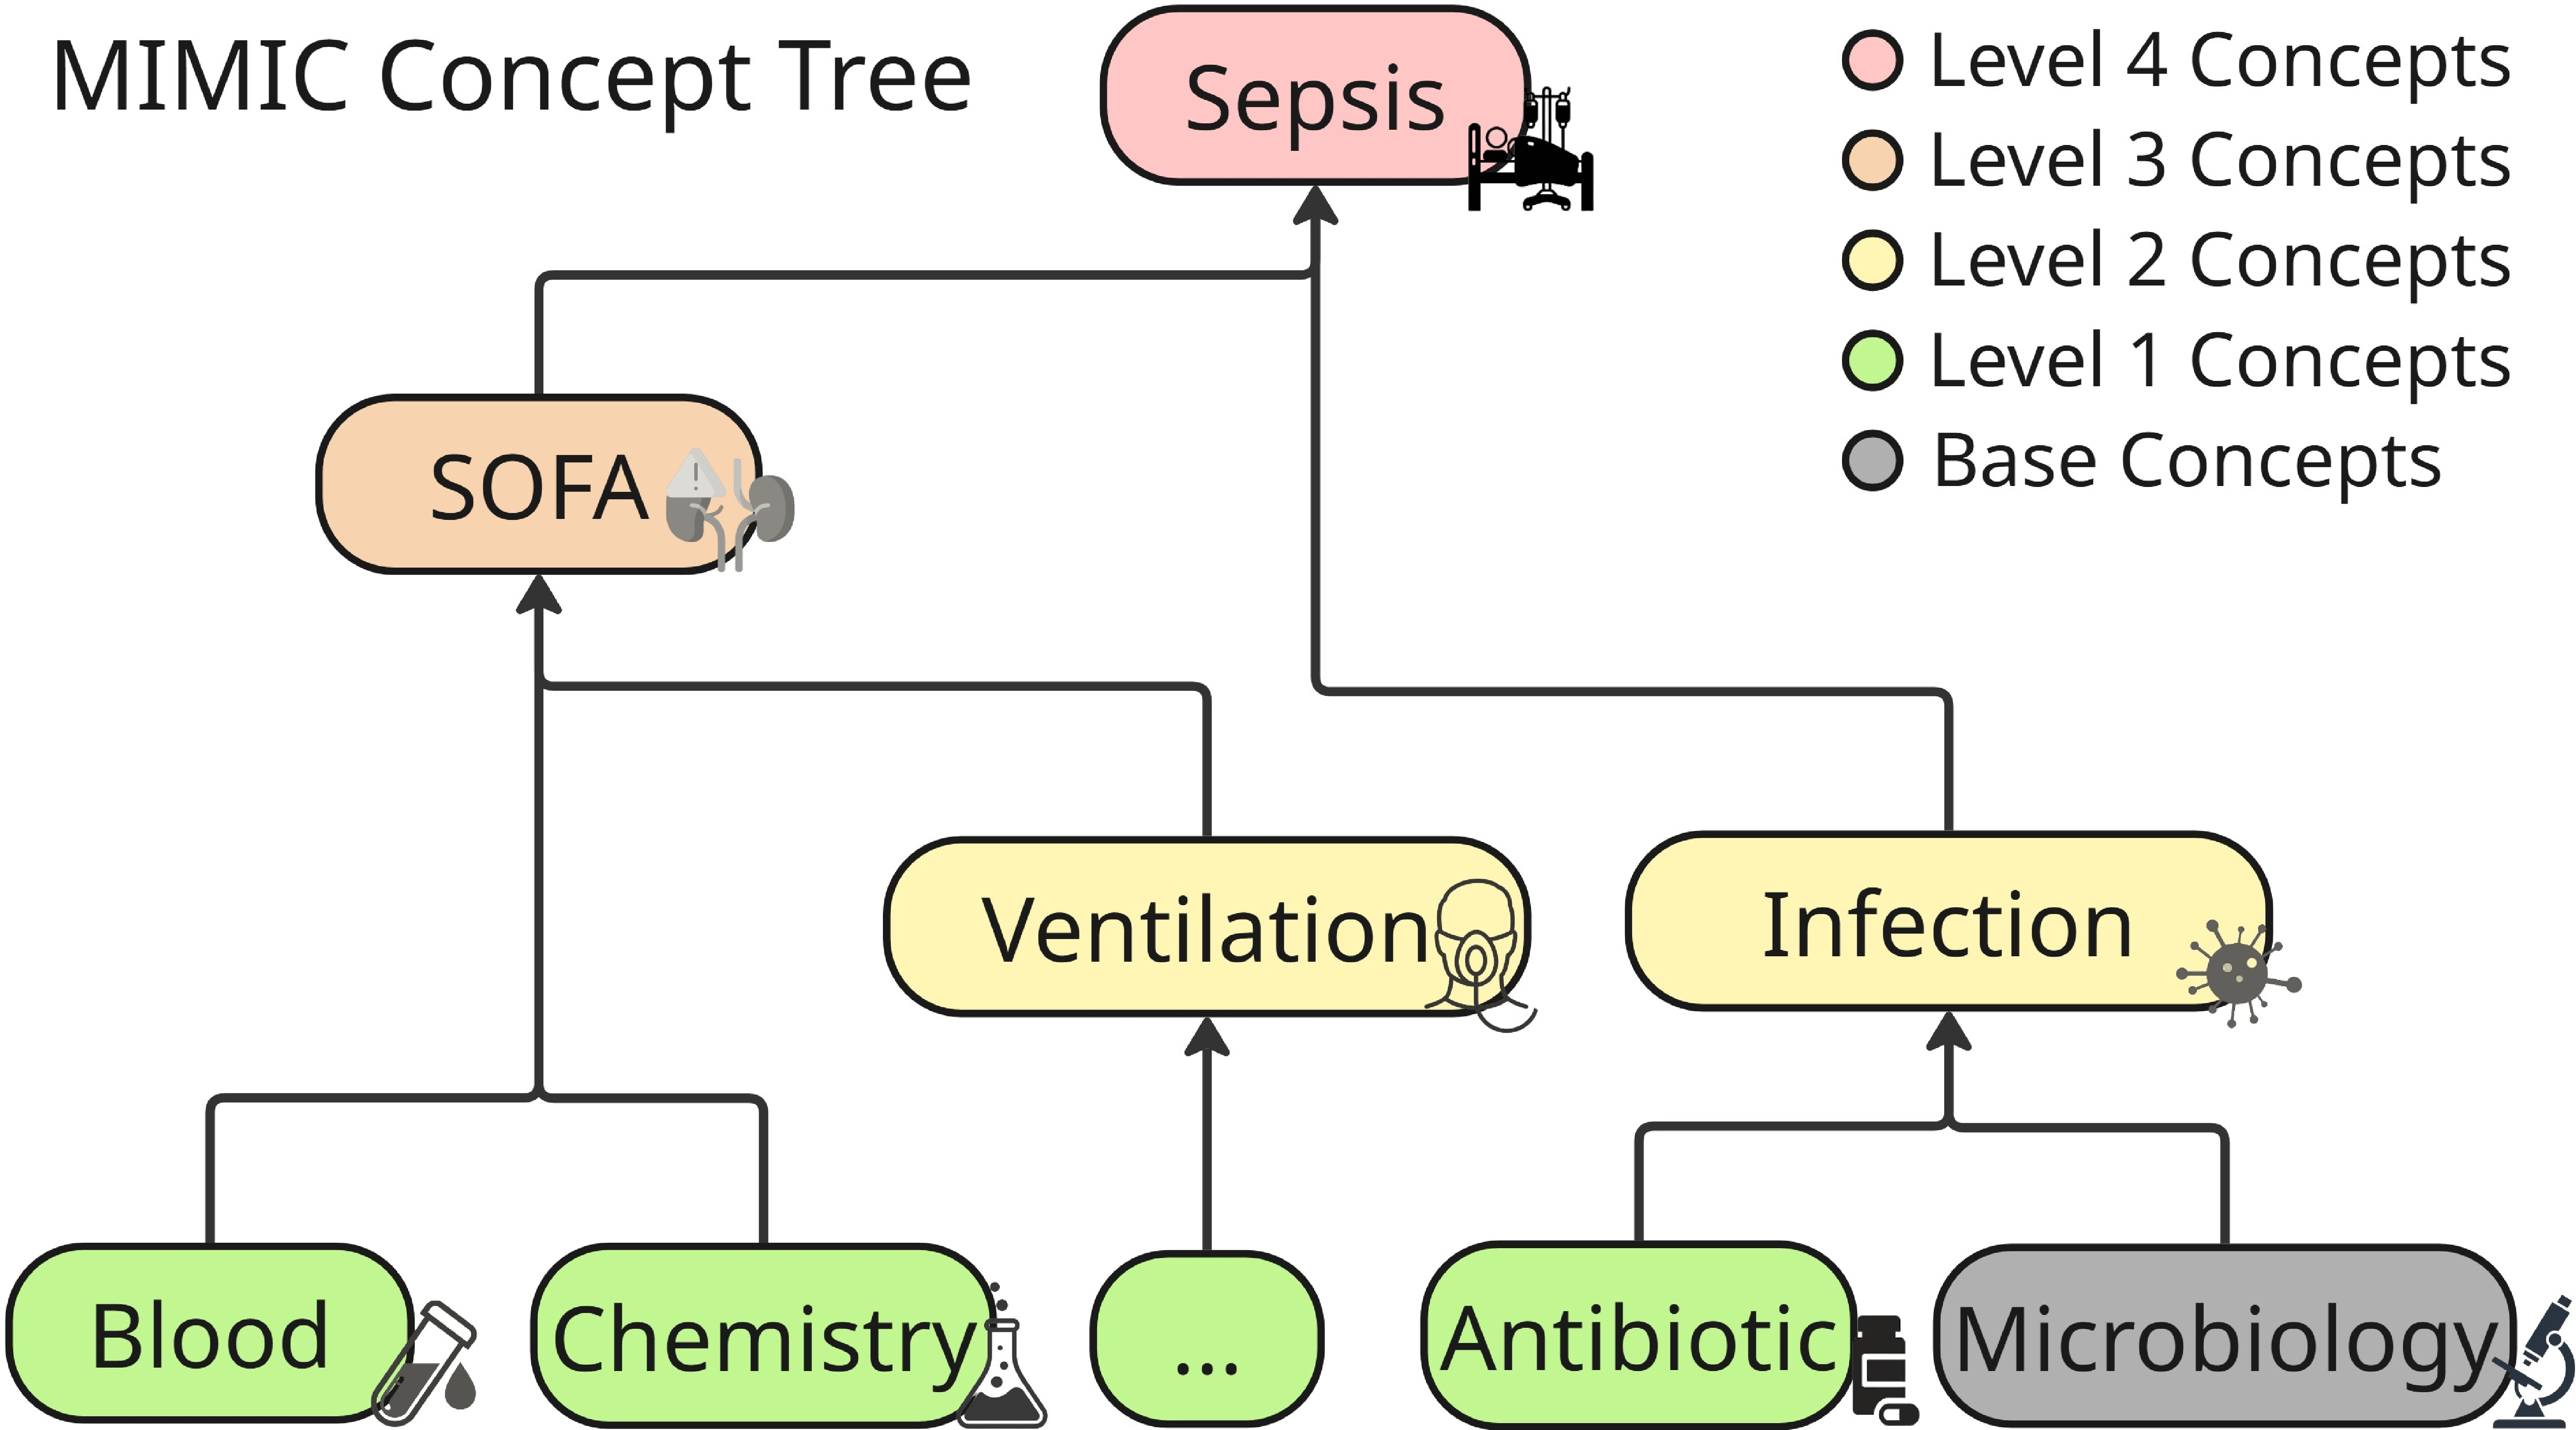
\includegraphics[width=\linewidth]{figures/dependency_example.pdf}
    \end{minipage}
    \begin{minipage}{0.48\linewidth}
        \centering
        \raisebox{13mm}{
            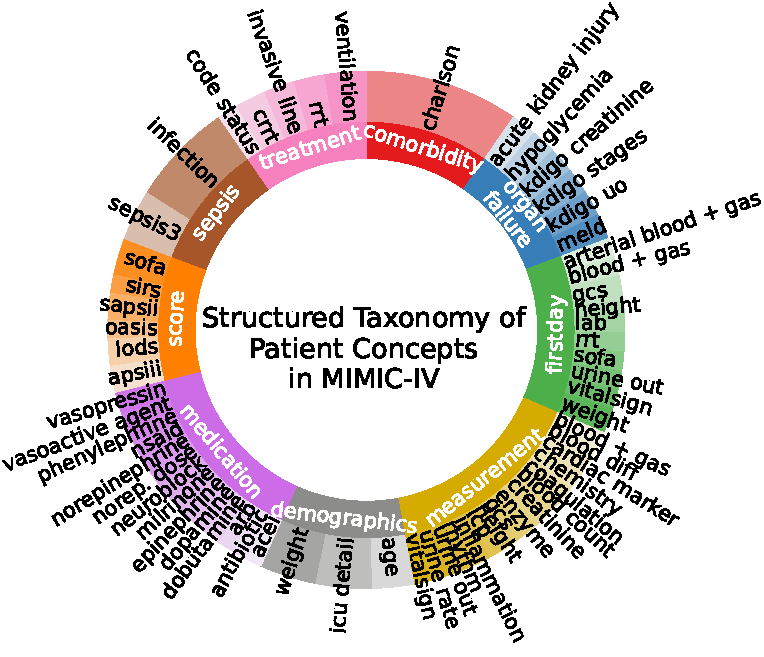
\includegraphics[width=\linewidth]{figures/concept_distribution.pdf}
        }
    \end{minipage}
    \vspace{-15mm}
    \caption{
    \textbf{Left:} Example dependency tree between clinical concepts in the MIMIC database for Sepsis. 
    Efficient sepsis monitoring involves recalculation of lower level concepts such as SOFA, Infection, etc. 
    \textbf{Right:} Structured taxonomy of all MIMIC concepts supercategories and corresponding concepts.
    }
    \label{fig:dependency_with_table}
\end{figure}
We constructed a clinical question answering benchmark grounded in the Medical Information Mart for Intensive Care IV (MIMIC-IV) database~\cite{johnson2023mimic}. All questions are derived from structured data in the MIMIC-IV \texttt{derived} schema, a curated collection of tables produced by community-validated SQL transformations applied to the raw MIMIC-IV data~\cite{johnson2021mimic}. The benchmark spans 63 clinical concepts covering nine physiological and pharmacological domains: comorbidity scoring, patient demographics, first-day assessments, laboratory measurements, medication administration, organ failure indices, severity scores, sepsis-related variables, and ICU treatments.

\paragraph{Concept Definition} Each concept corresponds to one derived table (e.g., \texttt{sofa}, \texttt{ventilation}, \texttt{kdigo\_stages}) and is defined programmatically as a set of question variants paired with ground-truth extraction functions. Each concept specifies (i) a base SQL query that joins the derived table with \texttt{mimiciv\_icu.icustays} and \texttt{mimiciv\_hosp.admissions} to produce a per-stay feature matrix, and (ii) a set of question variants, each targeting a distinct clinical attribute and question type. For each concept we also generate a structured natural-language guideline specification (defining clinical criteria, required measurements, and temporal windows) by synthesizing PubMed literature with an LLM (details in Appendix~\ref{app:guideline_gen}).

\paragraph{Clinical Knowledge Graph.}
Concepts are organized into a directed acyclic dependency graph $\mathcal{G} = (V, E)$, where an edge $(v_i, v_j)$ indicates that $v_j$ requires output from $v_i$. The graph is constructed by parsing SQL definitions in the MIMIC-Code repository and expanding with clinical conditions derived from ICD-10 diagnoses and UMLS Metathesaurus relations (see Appendix~\ref{app:knowledge_graph} for full construction details). This structure drives both difficulty stratification and compositional function reuse in our baseline pipeline.
\paragraph{Dependency-Based Difficulty} A key property of MIMIC-IV derived tables is that many are computed from other derived tables, inducing a directed acyclic dependency graph. We assign each concept a difficulty level equal to its longest dependency-chain depth in this graph. Concepts with no upstream dependencies (e.g., \texttt{vitalsign}, \texttt{gcs}, \texttt{norepinephrine}) are assigned \textit{Level 1}; these represent raw chart-level or medication-level extractions that require no multi-table reasoning. Concepts at depth 2 (e.g., \texttt{ventilation}, \texttt{creatinine\_baseline}, \texttt{first\_day\_lab}) are assigned \textit{Level 2}; they aggregate one layer of derived tables and correspond to clinically interpreted quantities. Concepts at depth 3 or greater (e.g., \texttt{sofa} at depth 3, \texttt{sepsis3} at depth 4) are grouped as \textit{Level 3+}; these composite scores integrate information across many physiological sub-systems and require reasoning over the most derived clinical constructs. This stratification provides a natural proxy for reasoning difficulty: correctly answering questions about a sepsis determination requires implicitly reasoning about organ dysfunction scores, infection likelihood, antibiotic timing, and microbiological culture data, a fundamentally more complex inference chain than answering questions about raw vital signs. We provide a visual representation of these dependencies in Figure \ref{fig:dependency_with_table}

% \paragraph{Question Types} We define question variants spanning four types for each concept. \textit{Binary} (yes/no) questions ask whether a clinical threshold is met or an event occurred (e.g., Does this patient have a SOFA score of 2 or more during their first 24 hours in the ICU?''). \textit{Numerical} questions require retrieving or computing a precise scalar value (e.g., What is this patient's minimum GCS score on their first ICU day?''). \textit{Temporal} questions test time-bounded reasoning by asking about measurements or events within a specific window relative to ICU admission (e.g., Was this patient's urine output rate below 0.5~mL/kg/hr within the first 6 hours of ICU admission?''); these are implemented via inline SQL \texttt{INTERVAL} expressions (6, 12, or 24 hours). \textit{Categorical} questions require predicting a discrete label from a multi-valued output space (e.g., Which ICU unit was this patient first admitted to?''). Across all 63 concepts, the benchmark contains 259 unique question phrasings (143 binary, 51 numerical, 58 temporal, 7 categorical).

\textbf{Sampling and Splits.} For each concept, up to 200 ICU stays are sampled per variant with class balance (100 positive / 100 negative for binary questions); no subject appears in more than one variant within a concept. A 10\% subset (20 rows per variant) forms the training split used during autoformalization; the remaining 90\% is the held-out test set. The full benchmark comprises \textbf{63,000 QA pairs} across 42,311 unique ICU stays (6,300 train / 56,700 test). Ground-truth labels are extracted deterministically from derived tables; missing values (e.g., no ICP measurements) are labeled \texttt{NaN} and a model correctly reporting data absence is scored correct.

\subsection{Longitudinal Reasoning}
{\color{blue}
We complement the static compositional QA benchmark with a longitudinal ICU surveillance task that evaluates whether an agent can maintain clinically consistent state over time rather than answer a single isolated question. The source cohort contains all MIMIC-IV ICU stays with length of stay at least 48 hours, yielding 46{,}337 stays and 602{,}381 checkpoint rows. We sample checkpoints every 4 hours from ICU admission through hour 48, so each trajectory contains 13 decision points. The public benchmark package is a held-out 2{,}000-stay subset (400 dev, 1{,}600 test; 26{,}000 checkpoints) selected from the cohort using a soft-balancing policy that preserves ICU heterogeneity while enriching rare high-acuity states.

\begin{figure}[t]
    \centering
    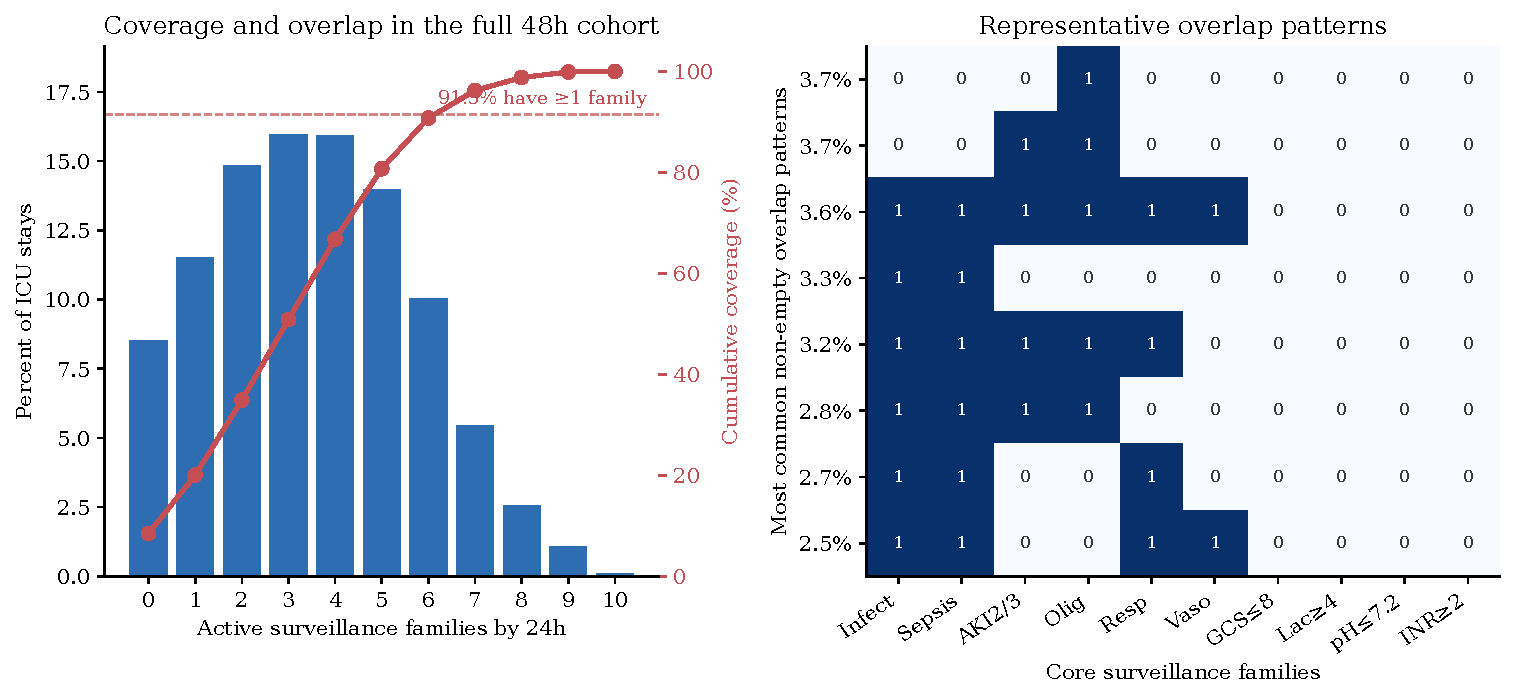
\includegraphics[width=\linewidth]{figures/surveillance_overlap_coverage.pdf}
    \caption{\textcolor{blue}{Coverage and overlap statistics for the longitudinal surveillance cohort. Left: distribution of the number of active core surveillance families by 24 hours among ICU stays with length of stay $\geq 48$ hours. Right: the most common non-empty overlap patterns across the ten core families, showing that many trajectories contain multiple concurrent monitoring problems rather than a single isolated disease.}}
    \label{fig:surveillance_coverage}
\end{figure}

Each checkpoint is labeled in two layers. Internally, we maintain a latent registry of 25 canonical ICU surveillance decisions spanning eight families: infection, sepsis, renal, respiratory, hemodynamic, neurologic, metabolic, and coagulation. Externally, these decisions are compressed into a simple agent output interface consisting of \texttt{suspected\_conditions}, \texttt{alerts}, \texttt{global\_action}, and \texttt{priority}. Importantly, these labels are not governed by a single one-time-trigger rule. Instead, the ground truth follows disease-appropriate checkpoint semantics derived from MIMIC-IV clinical principles: infection and sepsis are persistent episode states once they begin, AKI uses cumulative maximum-stage semantics, ventilation and vasoactive support are active-interval states, recent physiologic abnormalities such as lactate, pH, GCS, PF ratio, INR, and oliguria use recency-based TTL windows, and composite states such as septic shock are recomputed at every checkpoint from their component evidence.

\begin{figure}[t]
    \centering
    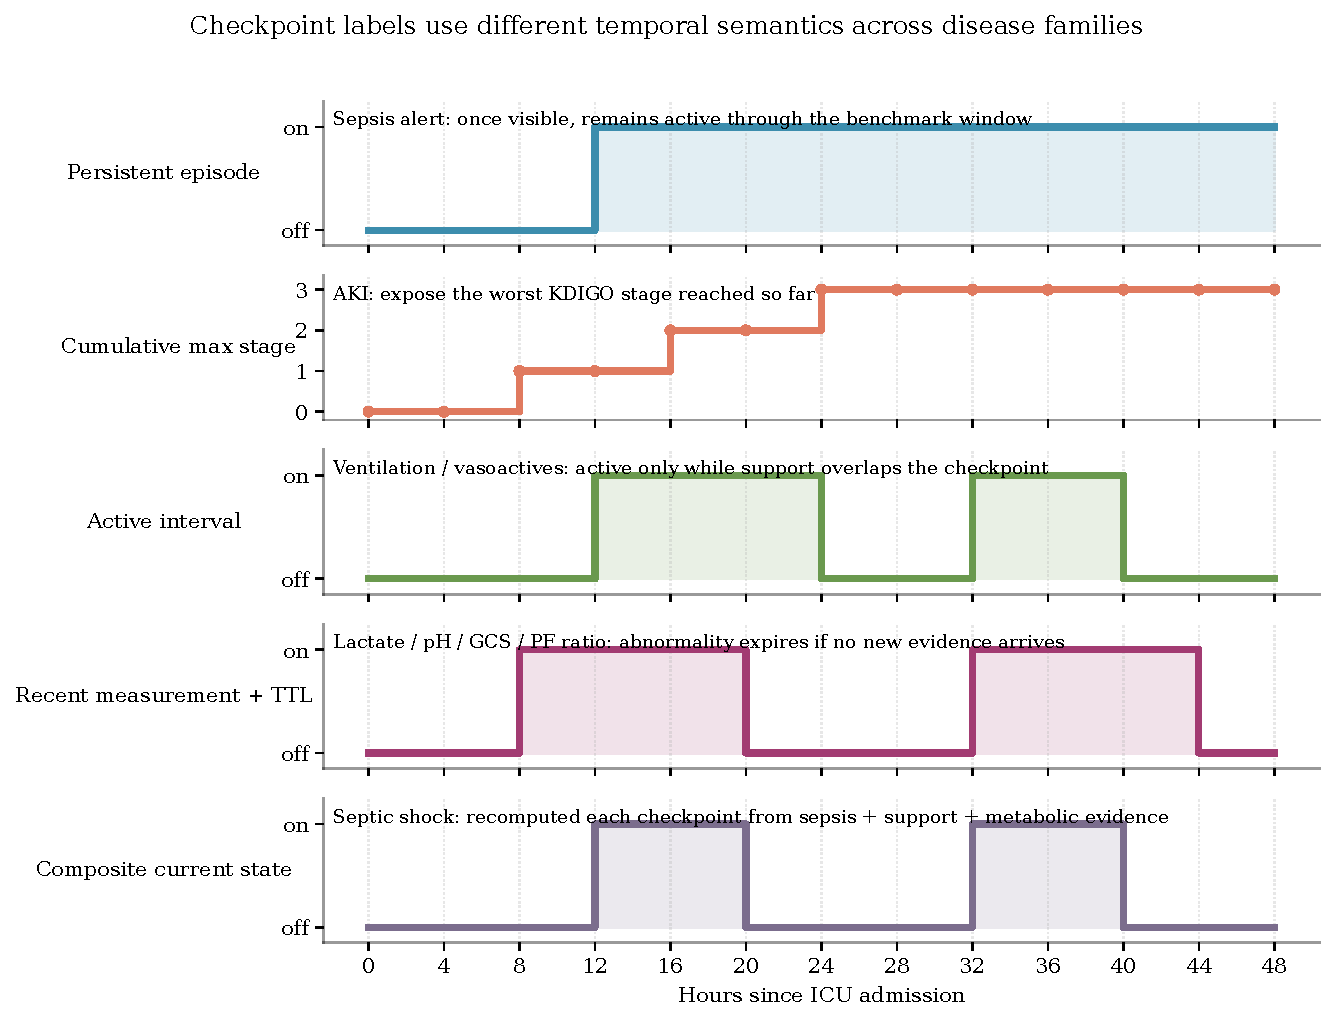
\includegraphics[width=\linewidth]{figures/surveillance_state_semantics.pdf}
    \caption{\textcolor{blue}{The longitudinal benchmark uses disease-dependent checkpoint semantics rather than a uniform once-positive-forever rule. Persistent syndromes such as sepsis remain active after onset; AKI tracks the worst KDIGO stage reached so far; support therapies such as ventilation and vasoactives are active only while the intervention overlaps the checkpoint; recent physiologic abnormalities such as lactate, pH, GCS, PF ratio, and oliguria expire after task-specific TTL windows; and composite states such as septic shock are recomputed from their component evidence at every checkpoint.}}
    \label{fig:surveillance_semantics}
\end{figure}

This temporal heterogeneity is a core source of difficulty. A model cannot solve the task by remembering a single binary label per disease. It must instead track which families persist once triggered, which families should decay when evidence becomes stale, and which families must be recomputed from multiple evolving components. For example, infection suspicion and Sepsis-3 onset remain active after they first occur within the 48-hour window; AKI is exposed as the worst KDIGO stage reached so far rather than the latest row value; invasive ventilation and vasoactive support are active only while the intervention overlaps the current checkpoint; oliguria and severe oliguria use rolling 6-hour and 24-hour windows; GCS states expire after 8 hours; blood-gas-derived states such as PF ratio, lactate, and acidemia expire after 12 hours; INR-based coagulation states expire after 24 hours; and septic shock or shock-with-hypoperfusion are recomputed from the conjunction of sepsis, support, and metabolic evidence. Figure~\ref{fig:surveillance_semantics} illustrates these distinct state-transition patterns.

This design makes the surveillance task both broad and genuinely longitudinal. In the full cohort, 91.49\% of stays activate at least one core surveillance family by 24 hours, 79.96\% activate at least two, and 65.10\% activate at least three; only 8.51\% remain negative across all ten core families at 24 hours (Figure~\ref{fig:surveillance_coverage}). The decision space also spans both common and rare ICU states. By 24 hours, for example, 51.23\% of stays meet Sepsis-3 criteria, 46.74\% receive invasive ventilation, 34.06\% receive vasoactive support, 17.33\% have PF ratio $<100$, 10.65\% have severe acidemia, and 1.91\% receive CRRT. To avoid a benchmark dominated by the most common alerts, the released 2{,}000-stay subset mixes 1{,}200 \emph{core-diversity} stays, 600 \emph{alert-enrichment} stays, and 200 \emph{low-signal} stays. This preserves realistic co-occurrence structure while ensuring enough support for thinner but clinically important heads such as AKI stage 3 (325 stays), septic shock (350), shock with hypoperfusion (280), severe acidemia (212), and severe coagulopathy (240).

At inference time, an agent is prompted at each checkpoint with the current hour, compact summary memory from prior steps, and access to one of two benchmark interfaces over the same time-bounded DuckDB session: a Python-session mode or a tool-first retrieval mode. In both cases the agent must retrieve any needed guideline or function evidence, infer the patient's current ICU state, emit a structured surveillance decision, and then summarize the step for future checkpoints. This setup turns longitudinal reasoning into an agentic state-tracking problem: the model must decide what clinical evidence to gather, how to interpret evolving partial observations, and when to escalate from monitoring to alerting without access to the full future trajectory.
}
